\documentclass[letterpaper,11pt,twoside]{article}
\usepackage{graphicx} % Required for inserting images
\usepackage[table,xcdraw,dvipsnames]{xcolor}
\usepackage{amsmath,amsfonts,amssymb,amsthm}
\usepackage{listings}
\usepackage{lipsum}
\usepackage{hyperref}
\usepackage{enumitem}

\usepackage{tikz}
\usepackage[siunitx, RPvoltages]{circuitikz}
\usetikzlibrary{3d}
\usepackage{comment}
\usepackage{caption,subcaption}
\usepackage{pgfplots}
\pgfplotsset{compat=newest} % or a newer version if available
\usepgfplotslibrary{groupplots}
\usetikzlibrary{pgfplots.groupplots}
\usetikzlibrary{shapes.geometric, arrows}
\tikzstyle{arrow} = [->,>=stealth,shorten >=2pt]
\newcommand{\re}[1]{\text{Re}\left(#1\right)}
\newcommand{\im}[1]{\text{Im}\left(#1\right)}
\newcommand{\bA}{\bm{A}}
\newcommand{\bB}{\bm{B}}
\newcommand{\bC}{\bm{C}}
\newcommand{\bE}{\bm{E}}
\newcommand{\bH}{\bm{H}}
\newcommand{\bD}{\bm{D}}
\newcommand{\bO}{\bm{0}}
\newcommand{\br}{\bm{r}}
\newcommand{\bk}{\bm{k}}
\newcommand{\bR}{\bm{R}}
\newcommand{\hA}{\hat{A}}
\newcommand{\hB}{\hat{B}}
\newcommand{\hC}{\hat{C}}
\newcommand{\ha}{\hat{a}}
\newcommand{\hn}{\hat{n}}
\newcommand{\hH}{\hat{H}}
\newcommand{\hN}{\hat{N}}
\newcommand{\hr}{\bm{\hat{r}}}
\newcommand{\hx}{\hat{x}}
\newcommand{\hX}{\hat{X}}
\newcommand{\hp}{\hat{p}}
\newcommand{\hS}{\hat{S}}
\newcommand{\hD}{\hat{D}}
\newcommand{\hy}{\hat{y}}
\newcommand{\hz}{\hat{z}}
\newcommand{\laplace}[1]{\mathscr{L}\left[#1\right]}
\newcommand{\ilaplace}[1]{\mathscr{L}^{-1}\left[#1\right]}
\newcommand{\fourier}[1]{\mathscr{F}\left[#1\right]}
\newcommand{\ifourier}[1]{\mathscr{F}^{-1}\left[#1\right]}
\newcommand{\ket}[1]{\left|#1\right\rangle}
\newcommand{\bra}[1]{\left\langle#1\right|}
\newcommand{\braket}[1]{\langle#1\rangle}
\newcommand{\D}{\mathcal{D}}
\usepackage{cancel}
\usepackage{bm}
\usepackage{fancyhdr}
\usepackage[utf8x]{inputenc}
\usepackage[T1]{fontenc}
\usepackage[margin=0.8in,top=1in,bottom=1in]{geometry}
%%%%%
\begin{filecontents*}{refs.bib}
@article{cohen1986quantum,
  title={Quantum mechanics, volume 1},
  author={Cohen-Tannoudji, Claude and Diu, Bernard and Laloe, Frank},
  journal={Quantum Mechanics},
  volume={1},
  pages={898},
  year={1986}
}
\end{filecontents*}
%
\newcommand{\institution}{University of Arizona}
\newcommand{\autor}{Nicolás Hernández Alegría}
\newcommand{\course}{OPTI 544 Quantum Optics}
\newcommand{\assignment}{Assignment 2}
%
\title{\textbf{\assignment}\\\course\\{\Large\institution}}
\author{\autor}
%\date{\today\\Total time: 12 hours}
%
\renewcommand{\sectionmark}[1]{\markright{#1}}
\fancypagestyle{mainstyle}{
    \fancyhf{} % Clear all header and footer fields
    \fancyfoot[C]{\thepage}
    \fancyhead[LE,RO]{\course} % Section name on odd pages
    \fancyhead[LO,RE]{\assignment}
    % Optional: Thin rules
    \renewcommand{\headrulewidth}{0pt} % Header rule
    \renewcommand{\footrulewidth}{0pt} % No footer rule
}
%
\begin{document}

\pagestyle{mainstyle}
\maketitle
%%
\section*{Exercise 1}
\begin{enumerate}[itemsep=0pt,topsep=0pt,parsep=0pt,label=\alph*)]
  \item The quadrature operators are:
  \begin{align*}
    \hX_1=\frac{\ha+\ha^\dagger}{2},\quad\text{and}\quad\hX_2=\frac{\ha-\ha^\dagger}{2i}.
  \end{align*}
  We can use them to express $\ha,\ha^\dagger$ in terms of $\hX_{1,2}$.
  \begin{align}
    \ha+\ha^\dagger&=2\hX_1\\
    \ha-\ha^\dagger&=2i\hX_2.
  \end{align}
  Then, 
  \begin{align*}
    (1)+(2):&\quad2\ha=2(\hX_1+i\hX_2)\longrightarrow\ha=\hX_1(0)+i\hX_2(0)\\
    (1)-(2):&\quad2\ha^\dagger=2(\hX_1-i\hX_2)\longrightarrow\ha^\dagger=\hX_1(0)-i\hX_2(0)
  \end{align*}
  Using these in the time-evolved quadrature operators:
  \begin{align*}
    \hX_1(t)&=\frac{\ha e^{-i\omega t}+\ha^\dagger e^{i\omega t}}{2}=\frac{[\hX_1(0)+i\hX_2(0)]e^{-i\omega t}+[\hX_1(0)-i\hX_2(0)]e^{i\omega t}}{2}\\
    \hX_1(t)&=\frac{e^{i\omega t}+e^{-i\omega t}}{2}\hX_1(0)+\frac{(e^{i\omega t}-e^{-i\omega t})}{2i}\hX_2(0)=\cos(\omega t)\hX_1(0)+\sin(\omega t)\hX_2(0).
  \end{align*}
  Likewise,
  \begin{align*}
    \hX_2(t)&=\frac{\ha e^{-i\omega t}-\ha^\dagger e^{i\omega t}}{2i}=\frac{[\hX_1(0)+i\hX_2(0)]e^{-i\omega t}-[\hX_1(0)-i\hX_2(0)]e^{i\omega t}}{2i}\\
    \hX_2(t)&=-\frac{e^{i\omega t}-e^{-i\omega t}}{2i}\hX_1(0)+i\frac{(e^{i\omega t}+e^{-i\omega t})}{2i}\hX_2(0)=-\sin(\omega t)\hX_1(0)+\cos(\omega t)\hX_2(0).
  \end{align*} 
  The commutation relation of the time-evolved quadrature operators is
  \begin{align*}
    [\hX_1,\hX_2]&=\frac{1}{4i}[\ha e^{-i\omega t}+\ha^\dagger e^{i\omega t},\ha e^{-i\omega t}-\ha^\dagger e^{i\omega t}]=\frac{1}{4i}\left\{-[\ha,\ha^\dagger]+[\ha^\dagger,\ha]\right\}=\frac{1}{4i}(-2)=\frac{i}{2}.
  \end{align*} 
  \item The expectation value is
  \begin{align*}
    \braket{\alpha|\hX_1(t)|\alpha}&=\braket{\alpha|\frac{\ha e^{-i\omega t}+\ha^\dagger e^{i\omega t}}{2}|\alpha}=\frac{1}{2}\left[\braket{\alpha|\ha|\alpha}e^{-i\omega t}+\braket{\alpha|\ha^\dagger|\alpha}e^{i\omega t}\right]=
    \frac{1}{2}\left[\alpha e^{-i\omega t}+\alpha^*e^{i\omega t}\right]\\
    &=\frac{1}{2}\left[(\alpha e^{-i\omega t})+(\alpha e^{-i\omega t})^*\right]=\re{\alpha e^{-i\omega t}}.\\
    \braket{\alpha|\hX_2(t)|\alpha}&=\braket{\alpha|\frac{\ha e^{-i\omega t}-\ha^\dagger e^{i\omega t}}{2i}|\alpha}=\frac{1}{2i}\left[\braket{\alpha|\ha|\alpha}e^{-i\omega t}-\braket{\alpha|\ha^\dagger|\alpha}e^{i\omega t}\right]=
    \frac{1}{2i}\left[\alpha e^{-i\omega t}-\alpha^*e^{i\omega t}\right]\\
    &=\frac{1}{2i}\left[(\alpha e^{-i\omega t})-(\alpha e^{-i\omega t})^*\right]=\im{\alpha e^{-i\omega t}}.
  \end{align*}
  The coherent state $\ket{\alpha e^{-i\omega t}}$ is a complex wave that rotates with a rate given by $\omega$. $\ket{\alpha}$ states the initial position in 
  the $\hX_1\hX_2$ phase space diagram.
  \begin{align*}
    \alpha e^{-i\omega t}=\braket{\hX_1}+i\braket{\hX_2}.
  \end{align*}

  The uncertainties requires also the expectation value of the operator squared:
  \begin{align*}
    \braket{\alpha|\hX^2_1(t)|\alpha}&=\frac{1}{4}\braket{\alpha|(\ha^2e^{-i2\omega t}+\ha\ha^\dagger+\ha^\dagger\ha+\ha^{\dagger2}e^{i2\omega t})|\alpha}=
    \frac{1}{4}\left[\alpha^2e^{-i2\omega t}+2|\alpha|^2+1+\alpha^{*2}e^{i2\omega t}\right]\\
    &=\frac{1}{4}\left[(\alpha e^{-i\omega t}+\alpha^*e^{i\omega t})^2+1\right]=\frac{1}{4}\left\{[2\re{\alpha e^{-i\omega t}}]^2+1\right\}.\\
    \braket{\alpha|\hX^2_2(t)|\alpha}&=-\frac{1}{4}\braket{\alpha|(\ha^2e^{-i2\omega t}-\ha\ha^\dagger-\ha^\dagger\ha+\ha^{\dagger2}e^{i2\omega t})|\alpha}=
    -\frac{1}{4}\left[\alpha^2e^{-i2\omega t}-2|\alpha|^2-1+\alpha^{*2}e^{i2\omega t}\right]\\
    &=\frac{1}{4}\left[1-(\alpha e^{-i\omega t}-\alpha^*e^{i\omega t})^2\right]=\frac{1}{4}\left\{1-[2i\im{\alpha e^{-i\omega t}}]^2\right\}.
  \end{align*}
  Uncertainty is 
  \begin{align*}
    \Delta\hX_1(t)&=\sqrt{\braket{\hX_1^2(t)}-\braket{\hX_1(t)}^2}=\sqrt{\frac{1}{4}\{[2\re{\alpha e^{-i\omega t}}]^2+1\}-[\re{\alpha e^{-i\omega t}}]^2 }=\sqrt{\frac{1}{4}}=\frac{1}{2}.\\
    \Delta\hX_2(t)&=\sqrt{\braket{\hX_2^2(t)}-\braket{\hX_2(t)}^2}=\sqrt{\frac{1}{4}\{1-[2i\im{\alpha e^{-i\omega t}}]^2\}-[\im{\alpha e^{-i\omega t}}]^2 }=\sqrt{\frac{1}{4}}=\frac{1}{2}.
  \end{align*}

  The diagram is shown below.
  \begin{figure}[htbp]
    \centering
    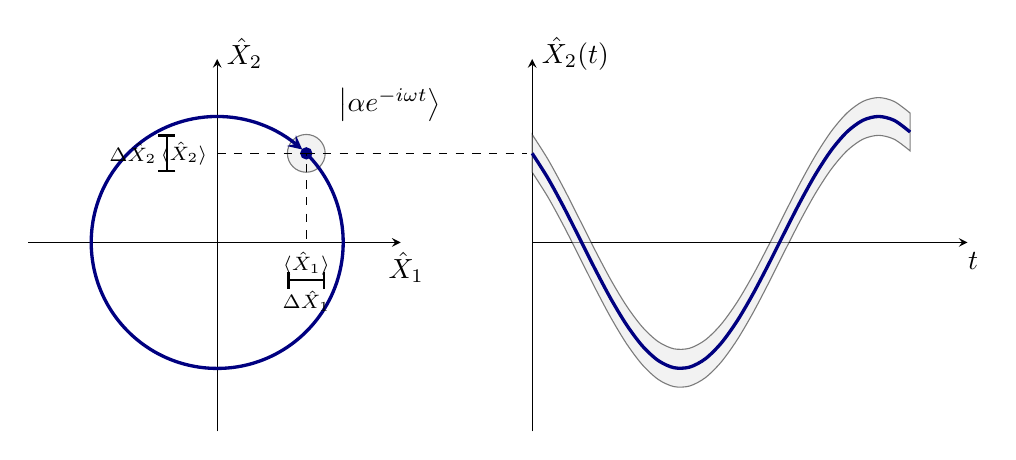
\begin{tikzpicture}[scale=.8]
      \draw[arrow](-3,0)--(3,0)node[below]{$\hX_1$};
      \draw[arrow](0,-3)--(0,3)node[right]{$\hX_2$};
      \draw[fill=gray!20,opacity=.5](45:2)+(0:.3)arc(0:360:.3);
      \draw[arrow,very thick,NavyBlue](0,0)+(45:2)node[circ,NavyBlue]{}arc(45:-315:2);
      \draw[dashed](0,{2*sin(45)})node[left,font=\scriptsize]{$\braket{\hX_2}$}--(45:2)--({2*cos(45)},0)node[below,font=\scriptsize]{$\braket{\hX_1}$}(45:2)--++(3.5,0);
      \draw(45:2.5)node[above right,black]{$\ket{\alpha e^{-i\omega t}}$};
      \draw[|-|,thick]({2*cos(45)-.3},-.6)--({2*cos(45)+.3},-.6)node[midway,below,font=\scriptsize]{$\Delta\hX_1$};
      \draw[|-|,thick](-.8,{2*sin(45)-.3})--(-.8,{2*sin(45)+.3})node[midway,left,font=\scriptsize]{$\Delta\hX_2$};
      \begin{scope}[xshift=5cm]
        \draw[arrow](0,0)--(7,0)node[below]{$t$};
        \draw[arrow](0,-3)--(0,3)node[right]{$\hX_2(t)$};
        \draw[fill=gray!20,opacity=.5]plot[domain=0:6, smooth, variable=\x]({\x},{2*sin(45-deg(\x))+.3})--
        plot[domain=6:0, smooth, variable=\x] ({\x}, {2*sin(45-deg(\x))-.3})--cycle;
        \draw[domain=0:6,smooth,variable=\x,NavyBlue,very thick]plot({\x},{2*sin(45-deg(\x))});
      \end{scope}
    \end{tikzpicture}
    \caption{Phase space of the coherent state and time-dependent quadrature operators.}
  \end{figure}
  \item The process is analogous. We know that 
  \begin{align*}
    \tilde{a}&=\hS^\dagger\hD^\dagger\ha\hD\hS=\cosh(r)\ha-e^{i\phi}\sinh(r)\ha^\dagger+\alpha,\quad\text{and}\\
    \tilde{a}^\dagger&=\hS^\dagger\hD^\dagger\ha^\dagger\hD\hS=\cosh(r)\ha^\dagger-e^{-i\phi}\sinh(r)\ha+\alpha^*.
  \end{align*}
  The expected value of $\hX_1(t)$ is 
  \begin{align*}
    \braket{\hX_1(t)}&=\braket{0|\hS^\dagger\hD^\dagger\frac{\ha e^{-i\omega t}+\ha^\dagger e^{i\omega t}}{2}\hD\hS|0}=\frac{1}{2}\braket{0|\tilde{a}e^{-i\omega t}+\tilde{a}^\dagger e^{i\omega t}|0}\\
    &=\frac{1}{2}\bra{0}\left[\cosh(r)\ha e^{-i\omega t}-e^{i\phi}\sinh(r)\ha^\dagger e^{-i\omega t}+\alpha e^{-i\omega t}+\cosh(r)\ha^\dagger e^{i\omega t}
    -e^{-i\phi}\sinh(r)\ha e^{i\omega t}+\alpha^*e^{i\omega t}\right]\ket{0}\\
    &=\frac{1}{2}[\alpha e^{-i\omega t}+\alpha^*e^{i\omega t}]\\
    \braket{\hX_1(t)}&=\re{\alpha e^{-i\omega t}}.
  \end{align*}
  Similarly,
  \begin{align*}
    \braket{\hX_2(t)}&=\braket{0|\hS^\dagger\hD^\dagger\frac{\ha e^{-i\omega t}-\ha^\dagger e^{i\omega t}}{2i}\hD\hS|0}=\frac{1}{2i}\braket{0|\tilde{a}e^{-i\omega t}+\tilde{a}^\dagger e^{i\omega t}|0}\\
    &=\frac{1}{2i}\bra{0}\left[\cosh(r)\ha e^{-i\omega t}-e^{i\phi}\sinh(r)\ha^\dagger e^{-i\omega t}+\alpha e^{-i\omega t}-\cosh(r)\ha^\dagger e^{i\omega t}
    +e^{-i\phi}\sinh(r)\ha e^{i\omega t}-\alpha^*e^{i\omega t}\right]\ket{0}\\
    &=\frac{1}{2}[\alpha e^{-i\omega t}-\alpha^*e^{i\omega t}]\\
    \braket{\hX_2(t)}&=\im{\alpha e^{-i\omega t}}.
  \end{align*}
  Doing the same for the operators squared:
  \begin{align*}
    \braket{\hX_1^2(t)}&=\braket{0|\hS^\dagger\hD^\dagger\left(\frac{\ha e^{-i\omega t}+\ha^\dagger e^{i\omega t}}{2}\right)^2\hD\hS|0}\\
    &=\frac{1}{4}\braket{0|\hS^\dagger\hD^\dagger\left(\ha e^{-i\omega t}+\ha^\dagger e^{i\omega t}\right)\hD\hS\hS^\dagger\hD^\dagger\left(\ha e^{-i\omega t}+\ha^\dagger e^{i\omega t}\right)\hD\hS|0}\\
    &=\frac{1}{4}\braket{0|(\tilde{a}e^{-i\omega t}+\tilde{a}^\dagger e^{i\omega t})^2|0}\\
    &=\frac{1}{4}\left[e^{-i2\omega t}\braket{0|\tilde{a}^2|0}+e^{i2\omega t}\braket{0|\tilde{a}^{\dagger2}|0}+\braket{0|\tilde{a}\tilde{a}^\dagger|0}+\braket{0|\tilde{a}^\dagger\tilde{a}|0}\right].
  \end{align*}
  We compute each term separately:
  \begin{align*}
    \braket{0|\tilde{a}^2|0}=&\braket{0|(\cosh(r)\ha-e^{i\phi}\sinh(r)\ha^\dagger+\alpha)(\cosh(r)\ha-e^{i\phi}\sinh(r)\ha^\dagger+\alpha)|0}\\
    =&\cosh^2(r)\braket{\ha^2}-e^{i\phi}\sinh(r)\cosh(r)\braket{\ha\ha^\dagger}+\alpha\cosh(r)\braket{\ha}-e^{i\phi}\sinh(r)\cosh(r)\braket{\ha^\dagger\ha}\\
    &+e^{i2\phi}\sinh^2(r)\braket{\ha^{\dagger2}}-\alpha e^{i\phi}\sinh(r)\braket{\ha^\dagger}+\alpha\cosh(r)\braket{\ha}-\alpha e^{i\phi}\sinh(r)\braket{\ha^\dagger}+\alpha^2\\
    &=\alpha^2-e^{i\phi}\sinh(r)\cosh(r)\\
    \braket{0|\tilde{a}^2|0}&=\alpha^2-\frac{1}{2}e^{i\phi}\sinh(2r).
  \end{align*}
  \begin{align*}
    \braket{0|\tilde{a}^{\dagger2}|0}=&\braket{0|(\cosh(r)\ha^\dagger-e^{-i\phi}\sinh(r)\ha+\alpha^*)(\cosh(r)\ha^\dagger-e^{-i\phi}\sinh(r)\ha+\alpha^*)|0}\\
    =&\cosh^2(r)\braket{\ha^{\dagger2}}-e^{-i\phi}\cosh(r)\sinh(r)\braket{\ha^\dagger\ha}+\alpha^*\cosh(r)\braket{\ha^\dagger}-e^{-i\phi}\sinh(r)\cosh(r)\braket{\ha\ha^\dagger}\\
    &+e^{-i2\phi}\sinh^2(r)\braket{\ha^2}-\alpha^*e^{-i\phi}\sinh(r)\braket{\ha}+\alpha^*\cosh(r)\braket{\ha^\dagger}-\alpha^*e^{-i\phi}\sinh(r)\braket{\ha^\dagger}+\alpha^{*2}\\
    =&\alpha^{*2}-e^{-i\phi}\sinh(r)\cosh(r)\\
    \braket{0|\tilde{a}^{\dagger2}|0}=&\alpha^{*2}-\frac{1}{2}e^{-i\phi}\sinh(2r).
  \end{align*}
  \begin{align*}
    \braket{0|\tilde{a}\tilde{a}^\dagger|0}=&\braket{0|(\cosh(r)\ha-e^{i\phi}\sinh(r)\ha^\dagger+\alpha)(\cosh(r)\ha^\dagger-e^{-i\phi}\sinh(r)\ha+\alpha^*)|0}\\
    \braket{0|\tilde{a}\tilde{a}^\dagger|0}=&\cosh^2(r)+|\alpha|^2.
  \end{align*}
  \begin{align*}
    \braket{0|\tilde{a}^\dagger\tilde{a}|0}=&\braket{0|(\cosh(r)\ha^\dagger-e^{-i\phi}\sinh(r)\ha+\alpha^*)(\cosh(r)\ha-e^{i\phi}\sinh(r)\ha^\dagger+\alpha)|0}\\
    \braket{0|\tilde{a}^\dagger\tilde{a}|0}=&\sinh^2(r)+|\alpha|^2.
  \end{align*}
  Putting all together:
  \begin{align*}
    \braket{\hX_1^2(t)}&=\frac{1}{4}\left\{[\alpha^2-\frac{1}{2}e^{i\phi}\sinh(2r)]e^{-i2\omega t}+[\alpha^{*2}-\frac{1}{2}e^{-i\phi}\sinh(2r)]e^{i2\omega t}+
    \cosh^2(r)+|\alpha|^2+\sinh^2(r)+|\alpha|^2\right\}\\
    &=\frac{1}{4}\left[(\alpha e^{-i\omega t}+\alpha^*e^{i\omega t})^2+\cosh(2r)-\sinh(2r)\cos(\phi-2\omega t)\right]\\
    \braket{\hX_1^2(t)}&=[\re{\alpha e^{-i\omega t}}]^2+\frac{1}{4}[\cosh(2r)-\sinh(2r)\cos(\phi-2\omega t)].
  \end{align*}
  The uncertainty is:
  \begin{align*}
    \Delta\hX_1(t)=\sqrt{\braket{\hX_1^2(t)}-\braket{\hX_1(t)}^2}=\frac{1}{2}\sqrt{\cosh(2r)-\sinh(2r)\cos(\phi-2\omega t)}.
  \end{align*}

  Similarly,
  \begin{align*}
    \braket{\hX_2^2(t)}&=\braket{0|\hS^\dagger\hD^\dagger\left(\frac{\ha e^{-i\omega t}-\ha^\dagger e^{i\omega t}}{2i}\right)^2\hD\hS|0}\\
    &=-\frac{1}{4}\braket{0|\hS^\dagger\hD^\dagger(\ha e^{-i\omega t}-\ha^\dagger e^{i\omega t})\hD\hS\hS^\dagger\hD^\dagger(\ha e^{-i\omega t}+\ha^\dagger e^{i\omega t})\hD\hS|0}\\
    &=-\frac{1}{4}\braket{0|(\tilde{a}e^{-i\omega t}-\tilde{a}^\dagger e^{i\omega t})^2|0}\\
    &=-\frac{1}{4}[e^{-i2\omega t}\braket{0|\tilde{a}^2|0}+e^{i2\omega t}\braket{0|\tilde{a}^{\dagger2}|0}-\braket{0|\tilde{a}\tilde{a}^\dagger|0}-\braket{0|\tilde{a}^\dagger\tilde{a}|0}].
  \end{align*}
  We use the previous results to get
  \begin{align*}
    \braket{\hX_2(t)}&=-\frac{1}{4}\left\{[\alpha^2-\frac{1}{2}e^{i\phi}\sinh(2r)]e^{-i2\omega t}+[\alpha^{*2}-\frac{1}{2}e^{-i\phi}\sinh(2r)]e^{i2\omega t}-
    \cosh^2(r)-|\alpha|^2-\sinh^2(r)-|\alpha|^2\right\}\\
    &=-\frac{1}{4}[(\alpha e^{-i\omega t}-\alpha^*e^{i\omega t})^2-\cosh(2r)-\sinh(2r)\cos(\phi-2\omega t)]\\
    \braket{\hX_2(t)}&=[\im{\alpha e^{-i\omega t}}]^2+\frac{1}{4}[\cosh(2r)+\sinh(2r)\cos(\phi-2\omega t)].
  \end{align*}
  And the uncertainty is:
  \begin{align*}
    \Delta\hX_2(t)=\sqrt{\braket{\hX_2^2(t)}-\braket{\hX_2(t)}^2}=\frac{1}{2}\sqrt{\cosh(2r)+\sinh(2r)\cos(\phi-2\omega t)}
  \end{align*}
  We can verify that $\Delta\hX_1(0)=e^{-r}/2$ and $\Delta\hX_2(0)=e^r/2$ when $\phi=t=0$.

  The phase space representation is shown below.
  \begin{figure}[htbp]
    \centering
    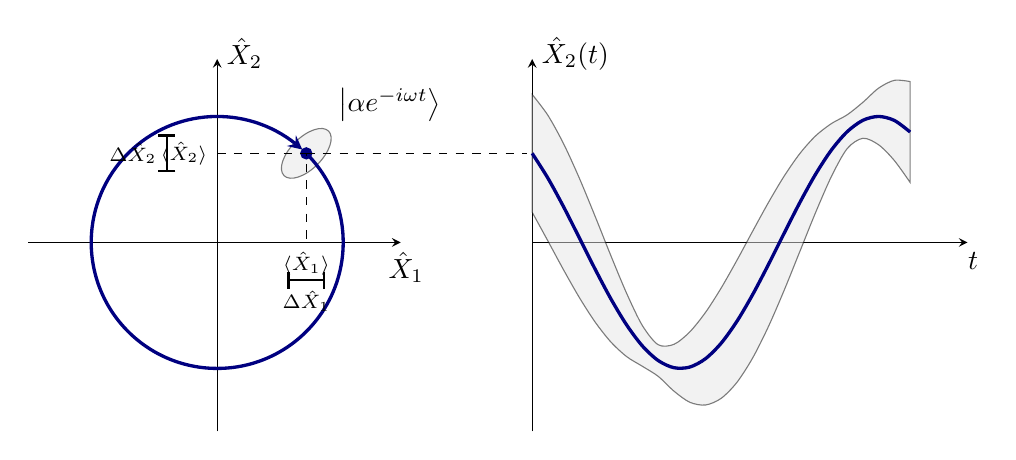
\begin{tikzpicture}[scale=.8]
      \def\r{.7}
      \def\w{1}
      \draw[arrow](-3,0)--(3,0)node[below]{$\hX_1$};
      \draw[arrow](0,-3)--(0,3)node[right]{$\hX_2$};
      \begin{scope}[shift={(45:2)}, rotate=45]
        \draw[fill=gray!20,opacity=.5] (0,0) ellipse (.5 and .25);
      \end{scope}
      %\draw[fill=gray!20,opacity=.5](45:2)+(0:.3)arc(0:360:.3);
      \draw[arrow,very thick,NavyBlue](0,0)+(45:2)node[circ,NavyBlue]{}arc(45:-315:2);
      \draw[dashed](0,{2*sin(45)})node[left,font=\scriptsize]{$\braket{\hX_2}$}--(45:2)--({2*cos(45)},0)node[below,font=\scriptsize]{$\braket{\hX_1}$}(45:2)--++(3.5,0);
      \draw(45:2.5)node[above right,black]{$\ket{\alpha e^{-i\omega t}}$};
      \draw[|-|,thick]({2*cos(45)-.3},-.6)--({2*cos(45)+.3},-.6)node[midway,below,font=\scriptsize]{$\Delta\hX_1$};
      \draw[|-|,thick](-.8,{2*sin(45)-.3})--(-.8,{2*sin(45)+.3})node[midway,left,font=\scriptsize]{$\Delta\hX_2$};
      \begin{scope}[xshift=5cm]
        \draw[arrow](0,0)--(7,0)node[below]{$t$};
        \draw[arrow](0,-3)--(0,3)node[right]{$\hX_2(t)$};
        \draw[fill=gray!20,opacity=.5]plot[domain=0:6,smooth,variable=\x]({\x},{2*sin(45-deg(\w*\x))+
        (0.5*sqrt( 0.5*(exp(2*\r)+exp(-2*\r))+0.5*(exp(2*\r)-exp(-2*\r))*cos(45-deg(2*\w*\x)) )) })--
        plot[domain=6:0, smooth, variable=\x]({\x},{2*sin(45-deg(\w*\x))-
        (0.5*sqrt( 0.5*(exp(2*\r)+exp(-2*\r))+0.5*(exp(2*\r)-exp(-2*\r))*cos(45-deg(2*\w*\x)) )) })--cycle;
        \draw[domain=0:6,smooth,variable=\x,NavyBlue,very thick]plot({\x},{2*sin(45-deg(\w*\x))});
      \end{scope}
    \end{tikzpicture}
    \caption{Phase space of the coherent state and time-dependent quadrature operators.}
  \end{figure}
\end{enumerate}


\clearpage
\nocite{*}
\bibliographystyle{plain}   % or unsrt, alpha, apalike, etc.
\bibliography{refs}

\end{document}
